\section{无限展开}
\label{sec:fvec-infinite-expansions}

有限维空间中，选定基以后，每个向量都由有限次加法和数乘精确地表示出来，坐标唯一，不涉及任何极限。进入无限维后，这一步分裂成两个问题：有限线性组合到底能覆盖哪些元素；对覆盖不到的元素，无穷多项的部分和能否趋于它，在什么意义下趋于它。数列的结构最简单，本节用数列把这两个问题分开研究，函数的正交展开要用到内积，在第~\ref{chap:function-inner-product-spaces}章讨论。

\subsection{代数基与级数表示}
\label{sec:fvec-algebraic-basis-series}

线性代数中的基只允许有限线性组合。把这一要求原样用于无限维空间，就得到下面的定义。

\begin{definition}[代数基]
\label{def:fvec-algebraic-basis}
设$V$是线性空间，$B\subseteq V$。若$B$中任意有限个不同元素线性无关，并且$V$的每个元素都是$B$中有限个元素的线性组合，称$B$为$V$的\term{代数基}（algebraic basis），也称\term{Hamel基}（Hamel basis）。
\end{definition}

定义中的两个条件各管一件事。线性无关保证表示唯一：若同一元素有两种有限表示，相减得到一个等于零的有限组合，各系数之差只能为零。“有限组合”则规定了允许的表示方式：不涉及任何极限，因此不需要事先给空间配上距离。

\paragraph{有限支撑数列与全体数列}
在$c_{00}$中，标准单位列$\{e_k\}_{k\geq1}$是代数基。线性无关上一节已经验证。若$x\in c_{00}$的非零项都在前$n$项之中，则
\[
 x=\sum_{k=1}^nx_ke_k
\]
是一个有限组合，所以$c_{00}$的每个元素都由$\{e_k\}$精确表示，坐标就是数列的各项。全体多项式$P$的情形相同：把多项式对应到它的系数列，$P$就成了换了名字的$c_{00}$，单项式$x^k$对应$e_{k+1}$。

同一族$\{e_k\}$在全体数列空间$\mathbb K^{\mathbb N_+}$中仍然线性无关，却不再张成整个空间。$e_1,\ldots,e_n$的任何组合从第$n+1$项起全为零，所以常数列$(1,1,\ldots)$不是有限个$e_k$的组合。$\{e_k\}$在$\mathbb K^{\mathbb N_+}$中只是一个线性无关族，它的有限组合恰好覆盖了$c_{00}$。

一般的无限维空间也有代数基，而且任何线性无关族都能扩充为一组代数基。证明要用到选择公理，具体通过Zorn引理进行，篇幅较长，读者可查阅线性代数或集合论的教材。这种存在性证明不给出具体的基，$\mathbb K^{\mathbb N_+}$的代数基至今没有可以写下来的公式。代数基仍然只允许有限组合，因此也不能用它谈论无穷和。

\paragraph{级数表示需要另外核对的内容}
要用$\{e_k\}$表示常数列这样的元素，自然想到写成无穷和$\sum_{k\geq1}x_ke_k$，把它理解为部分和
\[
 s_N=\sum_{k=1}^Nx_ke_k=(x_1,\ldots,x_N,0,0,\ldots)
\]
在$N\to\infty$时的极限。线性空间本身不提供极限，所以写下这个级数之前，先要规定“部分和趋于某个元素”的含义。

规定好收敛的意义之后，还要分别核对三件事。其一是收敛性：对给定的系数，部分和是否收敛。其二是表示范围：能够这样写出的元素是否覆盖整个空间。其三是唯一性：同一个元素能否有两组不同的系数。有限维时三者都自动成立，无限维时它们都依赖所选的收敛意义，需要逐项证明。

唯一性的失败最出乎意料，因为有限维中线性无关足以保证唯一。下面的例子采用逐项收敛的意义：对每个固定的$j$，第$j$项收敛。在数列空间中令
\[
 u_0=e_1,\qquad u_k=e_k-e_{k+1},\quad k\geq1.
\]

这族元素的任意有限个线性无关。设$a_0u_0+\sum_{k=1}^na_ku_k$是零数列。读第$n+1$项得$-a_n=0$；再依次读第$n$项、第$n-1$项直到第$2$项，由$a_k-a_{k-1}=0$得到$a_{n-1}=\cdots=a_1=0$；最后读第$1$项，得$a_0=0$。

然而$e_1$有两种展开。第一种就是$e_1=u_0$，系数列为$(1,0,0,\ldots)$。第二种来自逐项相消：前$N$个$u_k$之和是
\[
 \sum_{k=1}^Nu_k=e_1-e_{N+1},
\]
当$N\geq j$时，它的第$j$项等于$e_1$的第$j$项，所以逐项收敛到$e_1$，系数列为$(0,1,1,\ldots)$。在有限组合的意义下这族元素线性无关，在无穷和的意义下却有两种展开。

也不能默认每个无限维空间都有一族可数元素，使每个元素都能写成它们的级数。考虑有界数列，以两个数列各项之差的上确界衡量它们的距离。对$\mathbb N_+$的每个子集$S$，令$\chi_S$在$k\in S$处取$1$、其余取$0$。两个不同子集给出的数列在某一项相差$1$，所以彼此距离为$1$，这样的数列有不可数个。

假设某个可数族$\{u_j\}$能把每个有界数列都写成在这种距离下收敛的级数$\sum_ja_ju_j$。那么系数取有理数（复情形取实部、虚部都为有理数）的有限组合就构成一个可数集，并且能以任意精度逼近每个有界数列：先截断级数，再把系数换成相近的有理数。

于是以每个$\chi_S$为中心、半径$\tfrac12$的开球中都要有这个可数集的点。这些球两两不交，不可数个球却只分到可数个点，矛盾。具有可数稠密子集的空间称为可分空间，其一般定义见第~\ref{chap:topological-spaces}章。可数级数表示的存在，要求空间可分。

\subsection{展开的收敛}
\label{sec:fvec-expansion-convergence}

向量列有两种自然的“接近”方式。一种逐项比较：对每个固定的分量，误差都趋于零，称为逐项收敛。另一种统一比较：所有分量上误差的最大值趋于零。在$\mathbb K^d$中两者没有区别。设每个分量的误差都趋于零，给定$\varepsilon>0$，第$k$个分量从第$N_k$步起误差小于$\varepsilon$。取
\[
 N=\max\{N_1,\ldots,N_d\},
\]
从第$N$步起，全部$d$个分量同时误差小于$\varepsilon$。

这一步用到分量只有有限个，有限个数才一定有最大值。分量无穷多时，$N_k$可能没有上界，每个分量迟早对上，却没有一个共同的时刻。下面用两个数列的截断说明，这两种意义给出的结论可以不同。

\paragraph{常数列的截断}
取$x=(1,1,1,\ldots)$，部分和$s_N=(1,\ldots,1,0,0,\ldots)$保留前$N$项、其余置零。误差$x-s_N$的前$N$项为$0$，从第$N+1$项起全为$1$。

固定任意一项$k$，只要$N\geq k$，第$k$项的误差就是$0$，所以$s_N$逐项收敛到$x$。但所有项上误差的最大值是
\[
 \sup_{k\geq1}\lvert x_k-(s_N)_k\rvert=1,\qquad N=1,2,\ldots,
\]
不随$N$减小。每一项迟早都对，可“尚未对上的项”永远存在，只是向后移动。

\paragraph{调和数列的截断}
再取$y=(1,\tfrac12,\tfrac13,\ldots)$，作同样的截断$t_N=(1,\ldots,\tfrac1N,0,\ldots)$，逐项收敛同样成立。误差$y-t_N$的非零项是$\tfrac1{N+1},\tfrac1{N+2},\ldots$，其中最大的是第一项，所以
\begin{equation}
 \sup_{k\geq1}\lvert y_k-(t_N)_k\rvert=\frac1{N+1}\to0.
 \label{eq:fvec-harmonic-truncation}
\end{equation}
这里统一的误差也趋于零：尾部的各项本身在变小，截掉它们造成的误差随之变小。图~\ref{fig:fvec-truncation-error}并排画出了这两次截断。

\begin{BookInlineFigure}
  \centering
  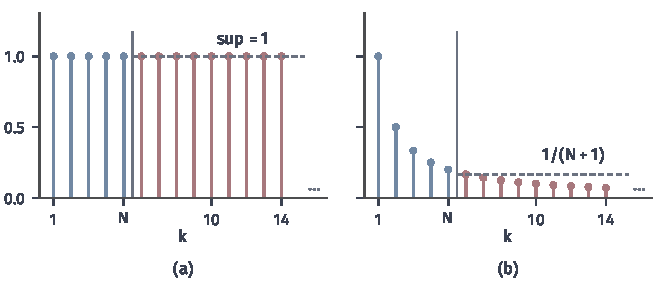
\includegraphics[width=112mm]{figures/04-spaces-measures-and-geometry/03-function-spaces/matplotlib/fvec-truncation-error/figure.pdf}
  \caption{同样的截断，不同的尾部。这里$N=5$，竖线左侧蓝色为保留的项，右侧红色为截掉的项，也就是误差，虚线标出误差的上确界。(a)常数列的尾部一直保持高度$1$，$N$增大时只是整体右移。(b)调和数列的尾部越来越低，上确界为$1/(N+1)$，随$N$增大而趋于零。}
  \label{fig:fvec-truncation-error}
\end{BookInlineFigure}

\paragraph{收敛意义的选择}
两个级数形式完全相同，都是$\sum_kx_ke_k$，区别只在系数。表~\ref{tab:fvec-truncation-compare}对比了两种误差给出的结论。在逐项收敛的意义下，每个数列都能这样展开；在统一误差的意义下，只有尾部趋于零的数列才能这样展开，也就是恰好$c_0$中的数列。所以“级数收敛”本身不是一个完整的陈述，必须说明用哪种误差衡量。

\begin{BookInlineTable}
  \centering
  \begin{tabular}{@{}lll@{}}
    \toprule
    误差的衡量方式 & $x=(1,1,1,\ldots)$ & $y=(1,\tfrac12,\tfrac13,\ldots)$\\
    \midrule
    逐项 & 收敛 & 收敛\\
    所有项的上确界 & 恒等于$1$，不收敛 & $1/(N+1)$，收敛\\
    \bottomrule
  \end{tabular}
  \caption{同一种截断在两种误差下的结论。}
  \label{tab:fvec-truncation-compare}
\end{BookInlineTable}

函数的情形相同，系数列$[1,1,\tfrac12,\tfrac16,\ldots]$就是一个例子。$e^x$的部分和是
\[
 s_N(x)=\sum_{k=0}^N\frac{x^k}{k!}.
\]
先在$[0,1]$上看误差。对$0\leq x\leq1$，把每个$x^k$放大到$1$，得到
\[
 0\leq e^x-s_N(x)=\sum_{k\geq N+1}\frac{x^k}{k!}\leq\sum_{k\geq N+1}\frac1{k!}.
\]

右边从$k=N+1$起，每一项不超过前一项的一半，所以用等比级数控制它：
\begin{equation}
 \sup_{0\leq x\leq1}\lvert e^x-s_N(x)\rvert\leq\frac{2}{(N+1)!}.
 \label{eq:fvec-exp-truncation}
\end{equation}
取$N=3$时，这个上界是$\tfrac1{12}$。所以在$[0,1]$上，统一误差趋于零。

换到整条实轴，结论就变了。在每个固定的$x$处，$s_N(x)$仍趋于$e^x$，因为这个幂级数处处收敛。但固定$N$后，对$x>0$有
\[
 e^x-s_N(x)\geq\frac{x^{N+1}}{(N+1)!},
\]
右边随$x\to+\infty$趋于无穷。所以每个$N$的统一误差都是无穷大，同一个级数在$\mathbb R$上逐点收敛、不一致收敛。

对一列近似函数，可以要求每个输入处的值收敛（逐点收敛），可以要求所有输入上的最大误差趋于零（一致收敛），也可以要求误差的积分趋于零。这三种意义互不等价。第~\ref{chap:function-normed-spaces}章用范数统一表达整体误差并比较这些收敛方式，具体表示及其截断误差则在第~\ref{chap:function-inner-product-spaces}章的正交展开和第~\ref{chap:function-approximation}章的函数逼近中研究。
